\documentclass[conference]{IEEEtran}
\IEEEoverridecommandlockouts
% The preceding line is only needed to identify funding in the first footnote. If that is unneeded, please comment it out.
\usepackage{cite}
\usepackage{amsmath,amssymb,amsfonts}
\usepackage{algorithmic}
\usepackage{graphicx}
\usepackage{textcomp}
\usepackage{xcolor}
\def\BibTeX{{\rm B\kern-.05em{\sc i\kern-.025em b}\kern-.08em
    T\kern-.1667em\lower.7ex\hbox{E}\kern-.125emX}}
\begin{document}

\title{Analyzing the Effects of Weather}
\author{
\IEEEauthorblockN{Erens, Sam}
\IEEEauthorblockA{
  \textit{Department of Mathematics} \\
  \textit{Department of Statistics} \\
  \textit{University of Illinois, Champaign} \\
  Champaign, IL, United States \\
  serens2@illinois.edu
}
\and
\IEEEauthorblockN{Hasson, Emily}
\IEEEauthorblockA{
  \textit{Department of Computer Science} \\
  \textit{Department of Statistics} \\
  \textit{University of Illinois, Champaign} \\
  Champaign, IL, United States \\
  ehasson2@illinois.edu
}
\and
\IEEEauthorblockN{Nelson, Lucas}
\IEEEauthorblockA{
  \textit{Department of Economics} \\
  \textit{Department of Statistics} \\
  \textit{University of Illinois, Champaign}\\
  Champaign, IL, United States \\
  lln2@illinois.edu}
}

\maketitle

\begin{abstract}
In this paper, we address the challenges in collecting, cleaning, and analyzing gigabytes of weather related data. Using archives of
\end{abstract}

\begin{IEEEkeywords}
spatiotemporal data, Apache Spark, model fitting
\end{IEEEkeywords}

\section{Introduction}

\begin{itemize}
  \item Describe the problem being solved and why it is important.
  \item Discuss your motivation for pursuing this problem.
  \item Clearly state what the features and model output will be.
  \begin{itemize}
    \item Note that these components can be reused from the project proposal paragraph.
  \end{itemize}
\end{itemize}

\section{Related Work}

\begin{itemize}
  \item Discuss published work that relates to your project.
  \item Emphasize how your approach will be similar or different from others.
\end{itemize}

We will be looking for a \textbf{\underline{minimum of 6}} scholarly works cited.

Three citations must originate from either a scholarly journal or are pre-prints on arXiv. Consider searching for articles using Google Scholar: \texttt{https://scholar.google.com/}. From there, click the “cite” button to automatically generate the appropriate citation from MLA, APA, or BibTex. That said, there is a preference for using BibLaTeX or natbib to avoid any bibliography formatting errors or mixing styles.

\section{Data}

\begin{itemize}
  \item What type of data is it (text/network/image/sound)?
  \item Who collected the data? \\

  \textbf{The data gathered for this project is provided by the National Oceanic and Atmospheric Administration (NOAA)\footnote{This data is publicly available for anyone to use under the following terms provided by the Dataset Source}, a government agency that collects an array of information pertaining to daily weather forecasts, severe storm warnings, and more climate-related instances.} \\

  \item How large is the data's size when uncompressed?
  \item How many records and features exist?
  \item Did you have to apply any pre-processing to the data?
  \begin{itemize}
    \item List any preprocessing steps
    \item e.g. Normalization, Tokenization, ...
  \end{itemize}
  \item Were any special steps required?
  \item What kind of training/validation(dev)/test split is expected?
  \item Show examples (if possible) of the data.
  \begin{itemize}
    \item For structured data, include the first 10 records.
    \item For text data, include a few unstructured entries.
    \item For image data, include a few images.
    \item For sound data, include the wav graph of the music file.
    \item And so on...
  \end{itemize}
\end{itemize}

Please include a reference to where the data set can be found. \textbf{This does not count toward the minimum of 6 works cited.}

\subsection{Preliminary Technical Details and Results}

\textbf{For points in this section, you must have \underline{at least one model fit} and described within the progress report.}

\begin{itemize}
  \item Describe in detail the proposed model.
  \item Explain how it works in general (or specifically with your data).
  \item Show preliminary results in:
  \begin{itemize}
    \item Summary tables:
    \begin{itemize}
      \item Classification should highlight precision, recall, and accuracy metrics.
      \item Regression should state the RMSE, MSE, or MAE.
    \end{itemize}
    \item Graphs

    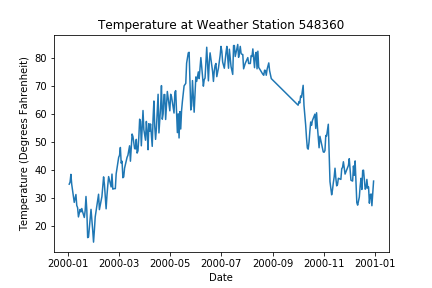
\includegraphics[scale=0.5]{./temperature.png}

    \textbf{The temperature at this weather station appears to peak in July at around 80 degrees Fahrenheit and drop to less than 20 degrees Fahrenheit in February. This suggests that this weather station is most likely located in the northern hemisphere.} \\

    \begin{itemize}
      \item Training and validation graphs based on the cost/loss function and evaluation metric (accuracy, F1, recall, RMSE, ...)
    \end{itemize}
  \end{itemize}
  \item Provide a timeline of the project to date and what the future work will entail.
  \begin{itemize}
    \item Summarize completed and future work by using a Gantt chart to break down the tasks and due dates.
    \begin{itemize}
      \item Break down each task by specifying \textbf{who} is \textbf{doing what} and \textbf{when} it will be done.
      \item Avoid saying ``Everyone in the group'' is working on a single task.
    \end{itemize}
  \end{itemize}
  \item Code
  \begin{itemize}
    \item Please provide code in a ZIP file or link to a GitHub repository. \textbf{Do \underline{not} submit your data set!}
    \item \textbf{If you have a private GitHub repository, please add @coatless.}
  \end{itemize}
\end{itemize}

\section{Contributions}

At the end of the progress report, please include a brief 1 - 2 sentence write-up of what each group member contributed to this stage of the project. Award each member with a percentage between 0 - 100 such that the sum of all percentages across group members will be equal to 100. \textbf{This section does not count toward the page limit.}

\section{Grading}

The project will be graded according to a rubric. There will be no possibility for resubmission. To avoid grading surprises, please speak with a member of course staff about your draft during Office Hours prior to turning it in.

\end{document}
